% 07_valutazione.tex — Capitolo 7: Valutare un modello: metriche e test.
% Documento didattico "Intelligenza artificiale nel progetto supervised_telemedicina".

\chapter{Valutare un modello: metriche e test}\label{cap:valutazione}

Nel capitolo~\ref{cap:training} abbiamo addestrato l'MLP e scelto la
configurazione migliore sulla loss di validazione. Ma come facciamo a sapere
se il modello è \emph{davvero} buono? In questo capitolo vediamo le metriche
di valutazione del progetto \progetto{}, implementate in
\file{training/metrics.py}, e i due test che il progetto usa per misurare
l'accuratezza in condizioni diverse. I numeri citati sono quelli reali del
report \file{data/models/report.json}.

\section{Perché l'accuracy da sola non basta}\label{sec:accuracy-insufficiente}

L'accuracy è la frazione di predizioni corrette: nel progetto,
$\frac{19702}{20000} = 0.9851$ sul test congelato. Sembra un ottimo numero,
ma da solo è fuorviante. Il problema è la \emph{distribuzione delle classi}:
se una classe è molto più frequente delle altre, un modello che predice
sempre quella classe ottiene un'accuracy alta senza imparare nulla.

L'analogia da programmazione: un test unitario che passa sempre non dice
nulla sulla correttezza del codice. Un classificatore che risponde sempre
\classe{basso} avrebbe un'accuracy pari alla frazione di campioni
\classe{basso} nel test (nel nostro caso $\frac{7220}{20000} = 0.361$, ma
in un dataset molto sbilanciato potrebbe superare 0.9) pur essendo
completamente inutile in clinica: non riconoscerebbe mai un paziente a
rischio \classe{alto}. Per questo il progetto valuta il modello con un
insieme di metriche complementari.

\section{La matrice di confusione}\label{sec:matrice-confusione}

La matrice di confusione è una tabella $3 \times 3$ in cui le righe sono le
classi \emph{reali} e le colonne le classi \emph{predette}: la cella
$(i, j)$ conta quanti campioni della classe $i$ sono stati predetti come
classe $j$. La diagonale contiene i successi, fuori diagonale gli errori.
La figura~\ref{fig:confusione} mostra la matrice del test congelato.

\begin{figure}[htbp]
  \centering
  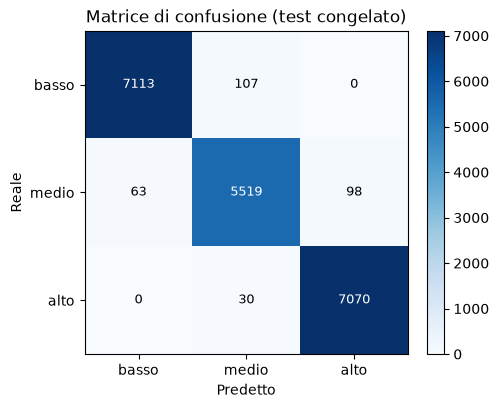
\includegraphics[width=0.85\textwidth]{figure/generate/confusione.png}
  \caption{Matrice di confusione sul test congelato (20000 campioni). La
  diagonale domina: 7113 + 5519 + 7070 = 19702 predizioni corrette su
  20000.}
  \label{fig:confusione}
\end{figure}

Leggiamo i numeri reali del report:

\begin{itemize}
  \item classe \classe{basso}: 7113 corretti, 107 confusi con
        \classe{medio}, 0 con \classe{alto};
  \item classe \classe{medio}: 5519 corretti, 63 confusi con
        \classe{basso}, 98 con \classe{alto};
  \item classe \classe{alto}: 7070 corretti, 30 confusi con
        \classe{medio}, 0 con \classe{basso}.
\end{itemize}

Due osservazioni. Primo, gli errori avvengono quasi solo tra classi
\emph{adiacenti} (\classe{basso}--\classe{medio} e
\classe{medio}--\classe{alto}): non esiste un solo caso in cui un
\classe{basso} venga predetto \classe{alto} o viceversa. Secondo, gli errori
più gravi dal punto di vista clinico sono i 30 \classe{alto} predetti come
\classe{medio}: sono i \emph{mancati} che le metriche di sicurezza del
progetto contano esplicitamente (capitolo~\ref{cap:sicurezza}).

\begin{esempio}{Leggere la matrice di confusione}
In \file{training/metrics.py} la matrice è costruita con un semplice ciclo:
\codice{matrice[vero, predetto] += 1}. La diagonale (\codice{np.trace}) dà
i successi; la somma per riga dà i reali per classe; la somma per colonna i
predetti per classe. Tutte le metriche delle sezioni seguenti derivano da
questi tre numeri.
\end{esempio}

\section{Precision, recall e F1 per classe}\label{sec:precision-recall-f1}

Per ogni classe $c$ si definiscono tre metriche:

\begin{itemize}
  \item \emph{precision}: $\frac{VP_c}{VP_c + FP_c}$, la frazione di
        predizioni di classe $c$ che sono corrette (quando il modello dice
        \classe{c}, quanto spesso ha ragione?);
  \item \emph{recall}: $\frac{VP_c}{VP_c + FN_c}$, la frazione di campioni
        reali di classe $c$ che vengono riconosciuti (quando un campione è
        \classe{c}, quanto spesso il modello lo trova?);
  \item \emph{F1}: la media armonica di precision e recall,
        $2 \cdot \frac{P \cdot R}{P + R}$.
\end{itemize}

Nel report del test congelato, per la classe \classe{alto}: precision
$0.9863$, recall $0.9958$, F1 $0.9910$. Il recall del \classe{alto} è la
metrica più importante in clinica: un paziente a rischio \emph{alto} non
riconosciuto è un paziente che non riceve l'attenzione necessaria. Il valore
$0.9958$ significa che su 7100 veri \classe{alto} il modello ne riconosce
7070 e ne perde 30. Le metriche di sicurezza del progetto
(\codice{metriche\_sicurezza} in \file{training/metrics.py}) contano
proprio questi mancati: \codice{mancati\_alto = 30} e
\codice{declassati\_critici = 30}. La distinzione tra precision e recall,
e il loro ruolo nella valutazione di classificatori, è trattata in modo
approfondito in \cite{hastie2009elements}.

\section{Il kappa di Cohen}\label{sec:kappa-cohen}

L'accuracy misura l'accordo tra modello e verità, ma una parte di quell'
accordo è dovuta al \emph{caso}: se le classi sono sbilanciate, due
classificatori indipendenti concordano per caso con probabilità non
trascurabile. Il \emph{kappa di Cohen} corregge proprio questo:

\begin{equation}
\kappa = \frac{p_o - p_e}{1 - p_e},
\end{equation}

dove $p_o$ è l'accordo osservato (l'accuracy) e $p_e$ l'accordo atteso per
caso, calcolato dai marginali della matrice di confusione. $\kappa = 1$
significa accordo perfetto, $\kappa = 0$ accordo pari al caso. Nel progetto
$\kappa = 0.9775$ sul test congelato: un accordo \emph{quasi perfetto} tra
l'MLP e le label del teacher. La funzione \codice{kappa\_cohen} in
\file{training/metrics.py} implementa la formula in numpy puro, senza
dipendenze esterne.

\section{Test congelato vs slice no-buffer}\label{sec:test-no-buffer}

Il progetto valuta il modello su due test diversi. Il \emph{test congelato}
è composto da 20000 campioni generati con seed 41 e mai toccati dal
training: è la valutazione ufficiale, fatta una sola volta. Ma questi
campioni sono stati generati con una \emph{buffer zone} attorno alle soglie
del teacher: i valori molto vicini a un confine (dove la classe è più
ambigua) sono stati esclusi dalla generazione. Il test congelato è quindi
leggermente ``facile''.

Per misurare la generalizzazione sui casi difficili, il progetto genera un
secondo test \emph{senza buffer} con la funzione
\codice{genera\_test\_no\_buffer} in \file{training/train\_model.py}:

\begin{lstlisting}[caption={Generazione del test senza buffer in \file{train\_model.py}.}]
def genera_test_no_buffer(seed_base: int, n_test: int) -> Tuple[np.ndarray, np.ndarray]:
    """Test aggiuntivo SENZA buffer zone (stesso seed del test congelato)."""
    X, y, _ = genera_batch(seed_base + 2, n_test, buffer_zone=False)
    return X, y
\end{lstlisting}

I risultati parlano chiaro:

\begin{itemize}
  \item test congelato (con buffer): accuracy $0.9851$, kappa $0.9775$;
  \item test no-buffer: accuracy $0.9324$, kappa $0.8959$.
\end{itemize}

La differenza ($0.9851$ vs $0.9324$) è l'\emph{ottimismo del test
bufferizzato}: sui campioni vicini alle soglie, dove il teacher stesso è
più ambiguo, l'MLP sbaglia di più. È un risultato importante da conoscere
quando si interpretano le metriche: l'accuracy sul test congelato è reale,
ma non va estrapolata ai casi limite.

\section{Dove sbaglia il modello}\label{sec:errori-modello}

La figura~\ref{fig:scatter-errori} mostra i 298 errori dell'MLP sul test
congelato, proiettati sul piano pressione sistolica $\times$ glicemia. Il
colore di ogni errore è la \emph{distanza dalle soglie} del teacher
(calcolata da \codice{distanza\_dalle\_soglie} in
\file{training/metrics.py}): una distanza piccola significa che il campione
è molto vicino a un confine di decisione.

\begin{figure}[htbp]
  \centering
  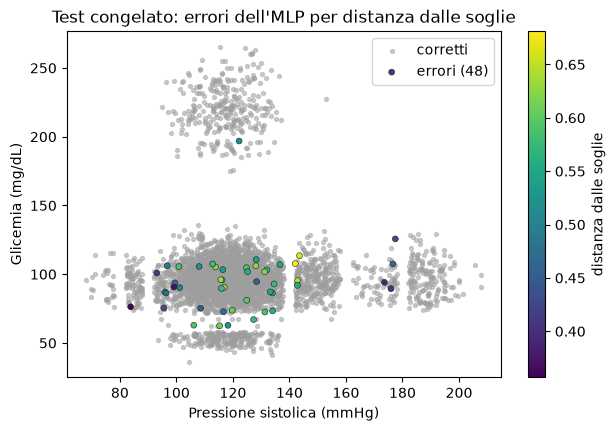
\includegraphics[width=0.85\textwidth]{figure/generate/scatter_errori.png}
  \caption{Errori dell'MLP sul test congelato (298 punti evidenziati),
  proiettati su pressione sistolica e glicemia. Il colore indica la distanza
  dalle soglie del teacher: gli errori si concentrano vicino ai confini.}
  \label{fig:scatter-errori}
\end{figure}

Il pattern è chiaro: gli errori \emph{cadono vicino ai confini}. La distanza
media degli errori dalle soglie è $0.524$ e la massima $0.681$: nessun
errore avviene lontano dai confini di decisione. È esattamente ciò che ci si
aspetta da un modello che approssima un teacher deterministico: dove il
teacher è netto, l'MLP impara bene; dove la classe cambia bruscamente (un
gradino), l'MLP, che produce confini curvi e morbidi, può sbagliare di una
classe.

\section{Il confronto con la baseline rule-based}\label{sec:baseline-rule-based}

Per interpretare correttamente l'accuracy serve un punto di riferimento: la
\emph{baseline rule-based}. La funzione \codice{baseline\_rule\_based} in
\file{training/train\_model.py} applica il teacher alle stesse 20000
feature del test congelato e confronta le sue label con quelle del dataset.
Il risultato nel report è \codice{accordo\_teacher\_label = 1.0} su
\codice{n\_campioni = 20000}.

Questo accordo perfetto è atteso per costruzione: le label del dataset sono
state generate dal teacher stesso. Ma è proprio il punto: la baseline
definisce l'\emph{upper bound di imitazione}. L'MLP non può fare meglio del
teacher, perché impara da lui; può solo avvicinarsi. L'accuracy di $0.9851$
va quindi letta come: l'MLP riproduce le regole del teacher nel $98.5\%$ dei
casi del test congelato. Come ricorda l'interpretazione del report, un'
accuracy alta qui significa \emph{buona approssimazione delle regole
sintetiche}, non accuratezza diagnostica su pazienti reali
\cite{progetto2026}.

\begin{esempio}{Perché la baseline è importante}
In un progetto di knowledge distillation la baseline rule-based è il
termine di paragone naturale: se l'MLP avesse un'accuracy molto inferiore
all'accordo del teacher, significherebbe che la distillazione ha perso
informazione. Il confronto con la baseline, insieme alle metriche di
sicurezza del capitolo~\ref{cap:sicurezza}, chiude il cerchio della
valutazione iniziata nel capitolo~\ref{cap:training}.
\end{esempio}